% Author: Henry Guo             *
% From: SJTU.CS.2               *
% Student ID: 516030910306      *
% Email: guohongyi@sjtu.edu.cn  *
% *******************************

\documentclass[12pt,a4paper]{article}
\usepackage{ctex}
\usepackage{amsmath,amscd,amsbsy,amssymb,latexsym,url,bm,amsthm}
\usepackage{epsfig,graphicx,subfigure}
\usepackage{enumitem,balance}
\usepackage{wrapfig}
\usepackage{mathrsfs,euscript}
\usepackage[usenames]{xcolor}
\usepackage{hyperref}
\usepackage[vlined,ruled,linesnumbered]{algorithm2e}
\hypersetup{colorlinks=true,linkcolor=black}

\DeclareGraphicsExtensions{.jpg,.pdf} % support .jpg

\newtheorem{theorem}{Theorem}
\newtheorem{lemma}[theorem]{Lemma}
\newtheorem{proposition}[theorem]{Proposition}
\newtheorem{corollary}[theorem]{Corollary}
\newtheorem{exercise}{Exercise}
\newtheorem*{solution}{Solution}
\newtheorem{definition}{Definition}
\theoremstyle{definition}

\renewcommand{\thefootnote}{\fnsymbol{footnote}}

\newcommand{\postscript}[2]
 {\setlength{\epsfxsize}{#2\hsize}
  \centerline{\epsfbox{#1}}}

\renewcommand{\baselinestretch}{1.0}

\setlength{\oddsidemargin}{-0.365in}
\setlength{\evensidemargin}{-0.365in}
\setlength{\topmargin}{-0.3in}
\setlength{\headheight}{0in}
\setlength{\headsep}{0in}
\setlength{\textheight}{10.1in}
\setlength{\textwidth}{7in}
\makeatletter \renewenvironment{proof}[1][Proof] {\par\pushQED{\qed}\normalfont\topsep6\p@\@plus6\p@\relax\trivlist\item[\hskip\labelsep\bfseries#1\@addpunct{.}]\ignorespaces}{\popQED\endtrivlist\@endpefalse} \makeatother
\makeatletter
\renewenvironment{solution}[1][Solution] {\par\pushQED{\qed}\normalfont\topsep6\p@\@plus6\p@\relax\trivlist\item[\hskip\labelsep\bfseries#1\@addpunct{.}]\ignorespaces}{\popQED\endtrivlist\@endpefalse} \makeatother

\begin{document}
\noindent

%========================================================================
\noindent\framebox[\linewidth]{\shortstack[c]{
\Large{\textbf{Lab02-Divide and Conquer}}\vspace{1mm}\\
CS214-Algorithm and Complexity, Xiaofeng Gao, Spring 2018.}}
\begin{center}

\footnotesize{\color{blue}$*$ Name: \underline{Hongyi Guo}\quad Student ID: \underline{516030910306}\quad Email: \underline{guohongyi@sjtu.edu.cn}}
\end{center}

\begin{enumerate}
\item
Assume that all elements of $A[1,\dots,n]$ are distinct and sorted, and $x$ is in $A$. Each element of $A$ is equally likely to be in any position in the array. Please give the average case analysis of Algorithm BinarySearch ($n=2^k$, $k\in\mathbb{N}$). The exact expression for the average number of comparisons $T(n)$ is required.
\begin{solution} Analyze.

\begin{enumerate}
\item The probability that we only need to compare \textbf{One} time is $\frac{1}{n}$. It's when $x$ is the middle element of the sequence $A$.
    $$(\cdots \underline{x_1}|\cdots)$$
\item The probability that we need to compare \textbf{Two} times is $\frac{2}{n}$. It's when $x$ is the middle element of the right or left half of $A$.
    $$(\cdots \underline{x_2}|\cdots x_1|\cdots \underline{x_2}|\cdots)$$
\item The probability that we need to compare \textbf{Three} times is $\frac{4}{n}$. It's when $x$ is in the position shown below.
    $$(\cdots \underline{x_3}|\cdots x_2|\cdots \underline{x_3}|\cdots x_1|\cdots \underline{x_3}|\cdots x_2|\cdots \underline{x_3}|\cdots)$$
\item $\cdots$
\end{enumerate}
So, the probability that we need to compare \textbf{i} times is $\frac{2^{i-1}}{n}$, $i\leq\log n=k$

Because the first $x_1$ actually belongs to the left half of the sequence $A$, there will be an additional element $A_n$ in the last of the right half. Thus, there is a probability of $1/n$ that we need to compare $k+1$ times.

The exact expression for the average number of comparisons $T(n)$ is:
$$T(n)=\sum\limits_{i=1}^{k}{i\times\frac{2^{i-1}}{n}}+\frac{k+1}{n}=1\times\frac{1}{n}+2\times\frac{2}{n}+\dots+k\times\frac{2^{k-1}}{n}+\frac{k+1}{n}$$.
$$2\times T(n)=1\times\frac{2}{n}+2\times\frac{4}{n}+\dots+k\times\frac{2^{k}}{n}+\frac{2(k+1)}{n}$$
$$T(n)=2\times T(n)-T(n)=-1\times\frac{1}{n}-1\times\frac{2}{n}-1\times\frac{4}{n}-\dots-1\times\frac{2^{k-1}}{n}+k\times\frac{2^k}{n}+\frac{k+1}{n}$$
$$=\frac{1-2^k}{n}+k\times\frac{2^k}{n}+\frac{k+1}{n}=\frac{(k-1)*2^k+1}{n}+\frac{k+1}{n}=\log n-1+\frac{\log n+2}{n}$$
\end{solution}

\item Given an integer array $A[1..n]$ and two integers $lower \le upper$, design an algorithm using divide-and-conquer method to count the number of ranges $(i,j)$ ($1 \leq i \leq j \leq n$) satisfying
$$
    lower \leq \sum_{k=i}^{j}{A[k]} \leq upper.
$$
\textbf{Example:}

Given $A = [1,-1,2]$, $lower = 1$, $upper = 2$, return 4.

The resulting four ranges are $(1,1)$, $(3,3)$, $(2,3)$ and $(1,3)$.

\begin{enumerate}
\item
Complete the implementation in the provided C/C++ source code {\color{blue}(The source code \emph{Code-Range.cpp} is attached on the course webpage)}.
\item
Write a recurrence for the running time of the algorithm and solve it by recurrence tree {\color{blue}(You can modify the figure source
\emph{Fig-RecurrenceTree.vsdx} to illustrate your derivation)}.
\begin{solution}
$$T(n)=2T(n/2)+O(n\log n)$$
\begin{figure}[htbp]
    \centering
    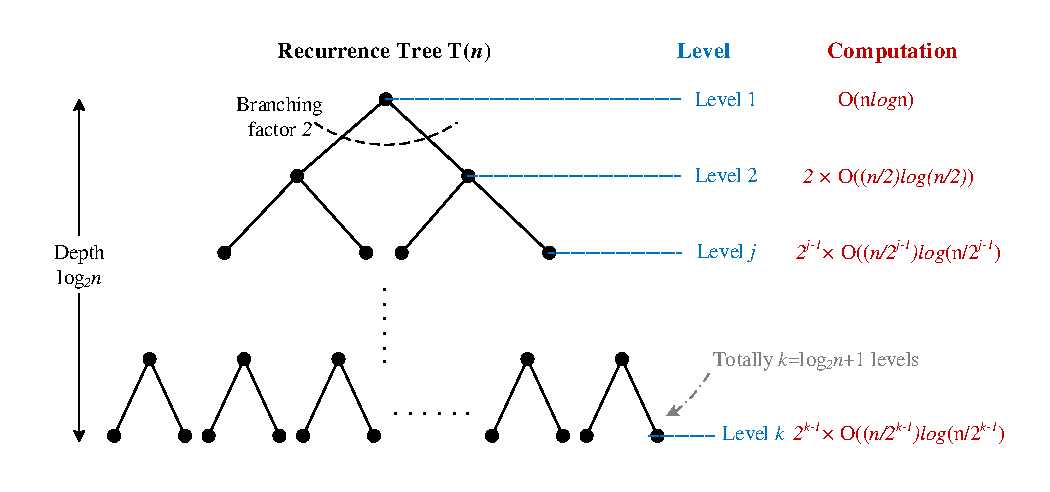
\includegraphics[width=0.8\textwidth]{Fig-RecurrenceTree.pdf}
    \caption{recurrence tree}\label{Fig-RecurrenceTree}
\end{figure}
\item
Complexity of $T(n)$=Sum up all computations at each level.

The total work done at the $j$-th level is
$$2^{j-1}\times O\left(\frac{n}{2^{j-1}}\log\frac{n}{2^{j-1}}\right)$$
The total work done is
$$\sum\limits_{j=1}^{\log_2n+1}2^{j-1}\times\left(\frac{n}{2^{j-1}}\log\frac{n}{2^{j-1}}\right)
=\sum\limits_{j=0}^{\log_2n}2^{j}\times\left(\frac{n}{2^{j}}\log\frac{n}{2^{j}}\right)
=\sum\limits_{j=0}^{\log_2n}n(\log n-j)$$
$$=(\log n+1)\times n\log n-n\times\frac{(\log n+1)\log n}{2}=\frac{n(\log n+1)\log n}{2}=O(n(\log n)^2)$$
So, $T(n)=O(n(\log n)^2)$.
\end{solution}
\item
{\color{red}{(Optional Sub-question with Bonus)}} Can we use the Master Theorem to solve the recurrence above? Please explain your answer.
\begin{solution}
No, we cannot use the Master Theorem to solve the recurrence above.

We can rewrite $T(n)$ as following
$$T(n)=2T(n/2)+O(n\log n)=2(T/2)+O(n*n^{\log_n(\log n)})=2(T/2)+O(n^{\log_n(\log n)+1})$$

Then we use Master Theorem.$a=2$, $b=2$, $d=\log_n(\log n)+1>1$.

As we can see, $a<b^d$. So, $T(n)=O(n^d)=O(n^{\log_n(\log n)+1})=O(n\log n)\neq O(n(\log n)^2)$.

The answer we get via Master Theorem is wrong. Thus, we cannot use Master Theorem in this case.
\end{solution}
\end{enumerate}

\item
\textbf{Transposition Sorting Network}: A comparison network is a \textbf{transposition network}  if each comparator connects adjacent lines, as in the network in Fig.~\ref{Fig-Transposition}.

\begin{figure}[htbp]
    \centering
    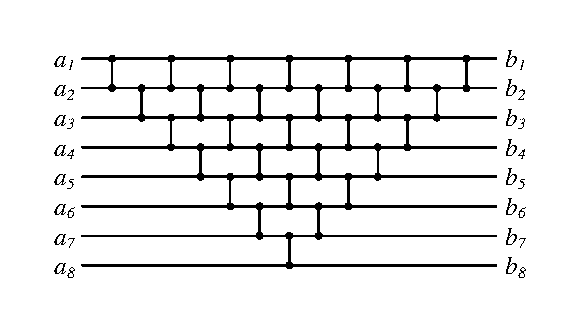
\includegraphics[width=0.5\textwidth]{Fig-Transposition.pdf}
    \caption{A Transposition Network Example}\label{Fig-Transposition}
\end{figure}

Prove that a transposition network with $n$ inputs is a sorting network if and only if it sorts the sequence $\langle n, n-1, \cdots, 1 \rangle$. {\color{blue}(Hint: Use an induction argument analogous to the \emph{Domain Conversion Lemma}.)}

\begin{proof}
% The problem is too difficult for me, I took about half a day to think but still can't solve it. I'm tied to the 0-1 principle.
% So I googled the answer and typed it. Now I'm sure that I've fully understood it.
\par
We prove the 'if' part first.

Define $A_a^i$ is the element in the $a$ line after the $i_{th}$ comparator when the input is sequence $A$.

We have the original sequence $D=\langle n,n-1,\dots,1\rangle$ and the normal sequence $A=\langle x_1,x_2,\dots,x_n\rangle$.

We can solve the problem by solving the claim that for any pairs of line $i$ and line $j$, if $i<j,D_i^k<D_j^k$ then $A_i^k\leq A_j^k$.

When $k=0$, it's obvious that $D_i^0>D_j^0$. The claim is true.

Now we assume the claim is true after the $k-1_{th}$ comparator and the $k_{th}$ comparator is between line $i$ and $i+1$. We should prove all of the pairs $(a,b)$ meets the claim, $a<b$.

\textbf{Case 1:} $a=i$ and $b=i+1$. It's obvious that $A_a^k\leq A_b^k$ because they are just compared and sorted.

\textbf{Case 2:} $a<i$ and $b>i+1$. Then $A_a^k=A_a^{k-1}$, $A_b^k=A_b^{k-1}$. The induction assumes that the $k-1_{th}$ comparator meets the claim, so does the $k_{th}$ comparator since the input elements are the same.

\textbf{Case 3:} $a<i$ and $b=i$. Then $D_a^k=D_a^{k-1}$, $A_a^k=A_a^{k-1}$, $D_b^k=\min\{D_i^{k-1},D_{i+1}^{k-1}\}$, $A_b^k=\min\{A_i^{k-1}, A_{i+1}^{k-1}\}$. If $D_a^k<D_b^k$, then $D_a^{k-1}<\min\{D_i^{k-1},D_{i+1}^{k-1}\}$. Because of the induction assume, $A_a^{k-1}\leq\min\{A_i^{k-1},A_{i+1}^{k-1}\}=A_b^k$. Thus, $A_a^k=A_a^{k-1}\leq A_b^k$.

\textbf{Case 4:} $a<i$ and $b=i+1$. Then $D_a^k=D_a^{k-1}$, $A_a^k=A_a^{k-1}$, $D_b^k=\max\{D_i^{k-1},D_{i+1}^{k-1}\}$, $A_b^k=\max\{A_i^{k-1}, A_{i+1}^{k-1}\}$. If $D_a^k<D_b^k$, then $D_a^{k-1}<\max\{D_i^{k-1},D_{i+1}^{k-1}\}$. Because of the induction assume, $A_a^{k-1}\leq\max\{A_i^{k-1},A_{i+1}^{k-1}\}=A_b^k$. Thus, $A_a^k=A_a^{k-1}\leq A_b^k$.

\textbf{Case 5:} $a=i$ and $b>i+1$. Then $D_a^k=\min\{D_i^{k-1},D_{i+1}^{k-1}\}$, $A_a^k=\min\{A_{i}^{k-1},A_{i+1}^{k-1}\}$, $D_b^k=D_b^{k-1}$, $A_b^k=A_b^{k-1}$. If $D_a^k<D_b^k$, then $\min\{D_i^{k-1},D_{i+1}^{k-1}\}<D_b^{k-1}$. Because of the induction assume, $\min\{A_i^{k-1},A_{i+1}^{k-1}\}\leq A_b^{k-1}=A_b^k$. Thus, $A_a^k=\min\{A_i^{k-1},A_{i+1}^{k-1}\}\leq A_b^k$

\textbf{Case 6:} $a=i+1$ and $b>i+1$. Then $D_a^k=\max\{D_i^{k-1},D_{i+1}^{k-1}\}$, $A_a^k=\max\{A_{i}^{k-1},A_{i+1}^{k-1}\}$, $D_b^k=D_b^{k-1}$, $A_b^k=A_b^{k-1}$. If $D_a^k<D_b^k$, then $\max\{D_i^{k-1},D_{i+1}^{k-1}\}<D_b^{k-1}$. Because of the induction assume, $\max\{A_i^{k-1},A_{i+1}^{k-1}\}\leq A_b^{k-1}=A_b^k$. Thus, $A_a^k=\max\{A_i^{k-1},A_{i+1}^{k-1}\}\leq A_b^k$

Thus we've prove our claim, so it's true that if a transposition network could sort $\langle n,n-1,\dots,1\rangle$, it's a sorting network.

Then we prove the `only if' part. It's obvious that if it cannot sort $\langle n,n-1,\dots,1\rangle$, then it's not a sorting network.

Together, a transposition network with $n$ inputs is a sorting network if and only if it sorts the sequence $\langle n, n-1, \cdots, 1 \rangle$.

\end{proof}
\end{enumerate}

%========================================================================
\end{document}
